\documentclass[aspectratio=169]{beamer}
\usepackage{amssymb,amsmath}
\usepackage{graphicx}
\usepackage{url}
\usepackage{color}
\usepackage{pagenote}[continuous,page]
\usepackage{cancel}   % Math "cancelto"
\usepackage{relsize}	% For \smaller
\usepackage{url}			% For \url
\usepackage{epstopdf}	% Included EPS files automatically converted to PDF to include with pdflatex

%For MindMaps
\usepackage{tikz}%
\usetikzlibrary{mindmap,trees,arrows}%

%%% Color Definitions %%%%%%%%%%%%%%%%%%%%%%%%%%%%%%%%%%%%%%%%%%%%%%%%%%%%%%%%%
%\definecolor{bordercol}{RGB}{40,40,40}
%\definecolor{headercol1}{RGB}{186,215,230}
%\definecolor{headercol2}{RGB}{80,80,80}
%\definecolor{headerfontcol}{RGB}{0,0,0}
%\definecolor{boxcolor}{RGB}{186,215,230}

%%% Save space in lists. Use this after the opening of the list %%%%%%%%%%%%%%%%
%\newcommand{\compresslist}{
%	\setlength{\itemsep}{1pt}
%	\setlength{\parskip}{0pt}
%	\setlength{\parsep}{0pt}
%}

%\setbeameroption{show notes on top}

% You should run 'pdflatex' TWICE, because of TOC issues.

% Rename this file.  A common temptation for first-time slide makers
% is to name it something like ``my_talk.tex'' or
% ``john_doe_talk.tex'' or even ``discrete_math_seminar_talk.tex''.
% You really won't like any of these titles the second time you give a
% talk.  Try naming your tex file something more descriptive, like
% ``riemann_hypothesis_short_proof_talk.tex''.  Even better (in case
% you recycle 99% of a talk, but still want to change a little, and
% retain copies of each), how about
% ``riemann_hypothesis_short_proof_MIT-Colloquium.2000-01-01.tex''?

\mode<presentation>
{
  \usetheme{CambridgeUS}
  \usecolortheme{dolphin}
  \useoutertheme{default}
  \useinnertheme{default}
  \setbeamercovered{invisible} % or whatever (possibly just delete it)
}
\beamertemplatenavigationsymbolsempty

\usepackage[english]{babel}
%\usepackage[latin1]{inputenc}
\usepackage{subfigure}

\usepackage{times}
\usepackage[T1]{fontenc}
\usepackage{CJKutf8}

%% makes the ppagenote command for figure references at the end.
\makepagenote
\renewcommand{\notenumintext}[1]{}
\newcommand{\ppagenote}[1]{\pagenote[Page \insertframenumber]{#1}}

\title[Experiment Design (01CH740)]{Experiment Design for Computer Sciences (01CH740)}
\author[Claus Aranha]{Claus Aranha\\{\footnotesize caranha@cs.tsukuba.ac.jp}}
\institute[U. Tsukuba]{University of Tsukuba, Department of Computer Sciences}


\subtitle[Experimental Factors]{Topic 08 - Statistical Recipes}
\date{}

\begin{document}

\begin{frame}
  \maketitle

  \vfill

  \hfill \tiny{Version 2023.1 (Updated \today)}
\end{frame}

\begin{frame}[t]{Outline}
  In this material we study a few extra topics related to statistical testing
  that came up in previous lectures.
\end{frame}

\section{Interaction Effects}

\begin{frame}{}

  \begin{center}
    {\large {\bf
        Second Order Interaction Effects
    }}
  \end{center}
  
\end{frame}

\begin{frame}[t]{What are Interaction Effects?}{}
  When analyzing data from an experiment, a common question of
  interest is {\bf how do the factors affect the response variable?}.\bigskip

  For example, we want to know how do the values of the parameters $F$
  and $CR$ affect the performance of the \emph{Differential Evolution}
  algorithm.\bigskip

  {\bf Main Effects} are how the factors individually affect the
  response variable:\footnote{hypothetical statements}
  \begin{itemize}
  \item Convergence time decreases as we increase the value of $CR$;
  \item Convergence time changes in a parabole with $F$, and is minimal when
    $F \approx 0.5$;
  \end{itemize}
  {\bf Interaction Effects} are how the factors affect the response
  variable in combination;
  \begin{itemize}
  \item When $CR \approx 0.5$, minimal convergence time happens for $F \approx 0.6$
  \item When $CR \approx 0.8$, minimal convergence time happens for $F \approx 1.1$
  \end{itemize}
\end{frame}

\subsection{Simple Example}
\begin{frame}{Simple Example -- Chocolate survey}

  Imagine that we are conducting a survey to discover what is the best
  food condiment.\bigskip

  We perform a survey, where we give the person a random food with a random condiment,
  and ask them their satisfaction.
  \begin{itemize}
  \item Independent Factor: {\bf Food:} Hotdog, Ice Cream
  \item Independent Factor: {\bf Condiment:} Chocolate Sauce, Mustard
  \item Response Variable : Enjoyment
  \end{itemize}

  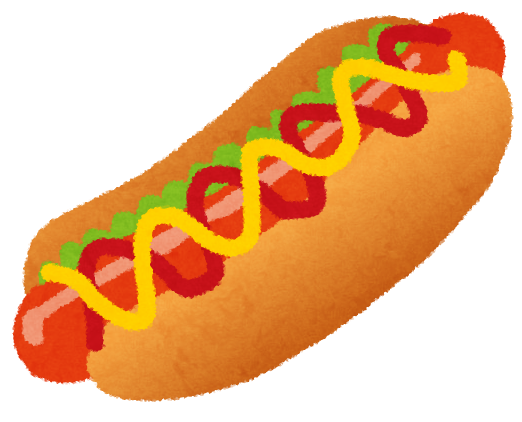
\includegraphics[width=0.2\textwidth]{../img/irasutoya_hotdog.png}
  \hfill
  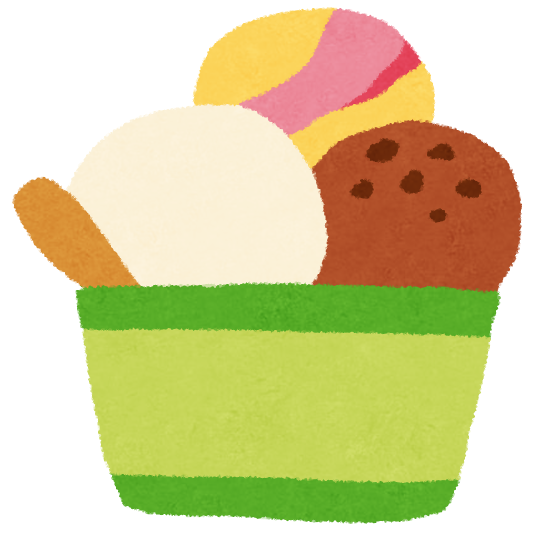
\includegraphics[width=0.2\textwidth]{../img/irasutoya_icecream.png}
  \ppagenote{Hotdog and icecream images from irasutoya}
\end{frame}

\begin{frame}[fragile]{Chocolate survey data}

  Here is what the data looks like (you can download data and code from manaba)\medskip

\begin{verbatim}
% cat Condiments.csv
"Enjoyment","Food","Condiment"
81.9269574232529,"Hot Dog","Mustard"
84.9397743293292,"Hot Dog","Mustard"
90.28647932801438,"Hot Dog","Mustard"
89.56180151665502,"Hot Dog","Mustard"
97.67682591880066,"Hot Dog","Mustard"
83.61712996934618,"Hot Dog","Mustard"
89.21086046510206,"Hot Dog","Mustard"
90.7668667221883,"Hot Dog","Mustard"
102.62044030772365,"Hot Dog","Mustard"
85.74390036422551,"Hot Dog","Mustard"
96.5923588947792,"Hot Dog","Mustard"
91.99449143926803,"Hot Dog","Mustard"
87.3332551483422,"Hot Dog","Mustard"
86.87685892829761,"Hot Dog","Mustard"
87.51938536071019,"Hot Dog","Mustard"
93.49125482138082,"Hot Dog","Mustard"
94.30378893191127,"Hot Dog","Mustard"
95.86999176797764,"Hot Dog","Mustard"
81.24348763821509,"Hot Dog","Mustard"
80.53783465646922,"Hot Dog","Mustard"
\end{verbatim}
\end{frame}

\begin{frame}[fragile]{Visualizing the results with a boxplot}
  At first glance, it seems that the condiment does not make a big
  difference?

  {\smaller
\begin{verbatim}
> satisfaction.df <- read.csv("Condiments.csv")
> boxplot(satisfaction.df$Enjoyment ~ satisfaction.df$Condiment)
\end{verbatim}}
  
  \begin{center}
    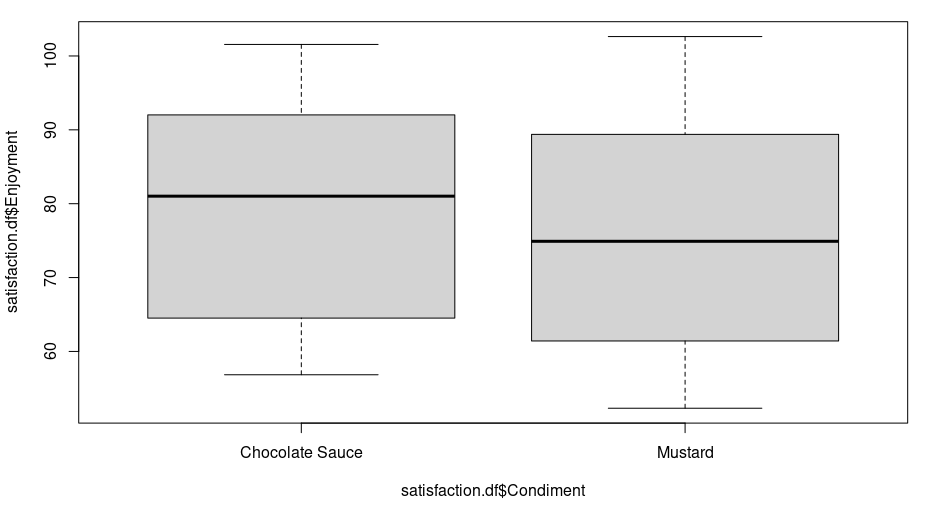
\includegraphics[width=0.65\textwidth]{../img/boxplot_condiment.png}
  \end{center}
\end{frame}

\begin{frame}[fragile]{Means across factors}{}
  We suspect that something is wrong here, so we plot the means for
  each combination of food and condiment.\footnote{It is always good
    to be curious about your data and explore it in depth.}\bigskip

  {\smaller
\begin{verbatim}
> aggregate(Enjoyment ~ Food + Condiment, satisfaction.df, mean)
       Food       Condiment Enjoyment
1   Hot Dog Chocolate Sauce  65.31661
2 Ice Cream Chocolate Sauce  93.04810
3   Hot Dog         Mustard  89.60569
4 Ice Cream         Mustard  61.30891
\end{verbatim}} \bigskip

    It appears that the Enjoyment depends on both the food and the
    condiment! Unfortunately, ice cream with mustard does not seem to
    be a very popular choice...
\end{frame}

\begin{frame}[fragile]{Measuring Interaction Effects}{}

  We can get a statistical measure of our interaction effect by using
  the ANOVA analysis on a linear model that includes the effect.

  {\smaller
\begin{verbatim}
> Food.lm <- lm(formula = Enjoyment ~ Food + Condiment + Food*Condiment, 
+               data = satisfaction.df)
> # ANOVA (effects of each factor on the final result)
> summary(aov(Food.lm))
               Df Sum Sq Mean Sq F value  Pr(>F)    
Food            1      2       2   0.064 0.80136    
Condiment       1    278     278  11.071 0.00135 ** 
Food:Condiment  1  15696   15696 626.153 < 2e-16 ***
Residuals      76   1905      25                    
---
Signif. codes:  0 ‘***’ 0.001 ‘**’ 0.01 ‘*’ 0.05 ‘.’ 0.1 ‘ ’ 1
\end{verbatim}}
    The F (and P) values on the Food:Condiment row indicate the strong interaction effect.

\end{frame}

\begin{frame}[fragile]{Visualization of Interaction Effects}{}

{\smaller
\begin{verbatim}
interaction.plot(satisfaction.df$Food, satisfaction.df$Condiment, 
                 satisfaction.df$Enjoyment, 
                 xlab = "Food", ylab = "Enjoyment", trace.label = "Condiment")
\end{verbatim}}

\begin{center}
  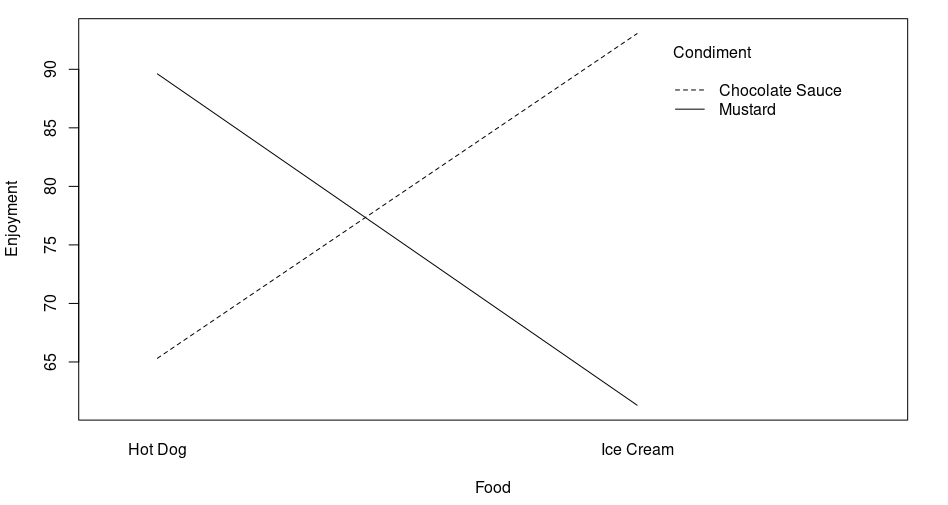
\includegraphics[width=0.7\textwidth]{../img/interactionplot_condiment.png}
\end{center}
\end{frame}

\subsection{Lung Cancer Example}
\begin{frame}{Another Example: Smoking, Abestos and Cancer}

  The data below was presented in Hilt et al. (1986), about the risk
  of lung cancer depending on whether a person smokes, and whether
  they are exposed to abestos.

  \begin{center}
    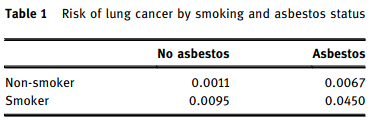
\includegraphics[width=0.55\textwidth]{../img/interaction_lungcancer.png}
  \end{center}\ppagenote{Lung Cancer table from VanderWeele and Know: A Tutorial on Interaction}

  We can observe that the risk of Lung Cancer increases much more when
  both Abestos and Smoking are present. More than we would expect from
  either factor alone.\bigskip

  Interaction effects can be both negative and positive.
\end{frame}

% TODO: Improve understanding of additive and multiplicative interaction effects

%\begin{frame}{Measuring Interaction}
%  - Additive Effects
%  - Multiplicative Effects (Ratio Effects)
%  
%  Which to use? Difficult question. There is always ``some'' interaction, if both
%  variables have an effect on the outcome. Better look at both, and consider the
%  characteristics and motivation of the experiment.
%\end{frame}



\subsection{Interaction Effects on DE}

\begin{frame}{Interaction Effects on DE Parameters}{}
  Let's see a more complex example, that is closer to computer science.\bigskip

  {\bf Differential Evolution} (DE) is a popular meta-heuristic algorithm
  that can be used to solve blackbox optimization problems.\bigskip

  The it is known that the performance of DE depends on the problem
  being solved, as well as its two control parameters: $F$ and
  $Cr$. Therefore, the user is encouraged to {\bf fine tune} the
  algorithm prior to application.\bigskip

  In this example, we run a simplified experiment to find optimal
  parameter values for DE for a sample problem.
\end{frame}

\begin{frame}[t]{DE Description}{}
  Differential Evolution is an algorithm that rely on two parameters:
  \begin{itemize}
  \item CR: Ranges from 0 to 1, recommended value is 0.5;
  \item F: Ranges from 0 to 2, recommended value is 0.8;
  \end{itemize}\bigskip

  It is recommended that the algorithm is fine-tuned for specific
  problems. In this case, we will use check the performance of the
  algorithm in a benchmark function under different parameter values.
\end{frame}

\begin{frame}[t]{Experimental Design}{}

  Scientific inquiry: Understand how the convergence rate of DE
  changes as we set different values of the parametes CR and F. In
  specific, try to detect if there are any interactions between these
  parameters.\bigskip
  
  \begin{itemize}
  \item {\bf Response Variable}: Number of iterations until a target solution quality is reached.
  \item {\bf Independent Factor 1}: CR, levels: 0.1, 0.3, 0.5, 0.7, 0.9
  \item {\bf Independent Factor 2}: F, levels: 0.2, 0.4, 0.8, 1.0, 1.2
  \item {\bf Noise Factor}: Random seed (probabilistic algorithm)
  \end{itemize}
  \bigskip

  Since this is an exploratory experiment, we do not set specific
  values for $\alpha$, $\beta$, etc. These values should be set when
  specific null and alternate hypothesis are considered.  
\end{frame}


\begin{frame}[t]{Initial observation of the parameters -- CR}{}
  First, let's observe how changing the parameters affect the response variable:
  \begin{columns}
    \column{0.4\textwidth}
    Notes:
    \begin{itemize}
    \item This is a box plot of the response value, grouped by CR value.
    \item It includes different values of F in the results, so
      interaction effects might be a concern.
    \item Still, we see a generally downwards trend for higher CR values {\bf For this problem}.
    \end{itemize}
    \column{0.6\textwidth}
    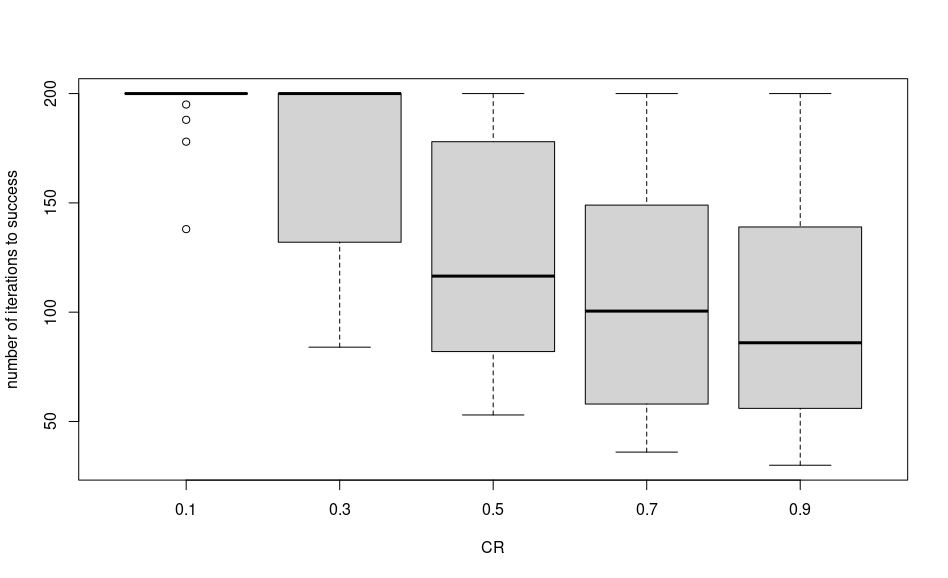
\includegraphics[width=\textwidth]{../img/DE_experiment_CR_analysis.png}
  \end{columns}
\end{frame}

\begin{frame}[t]{Initial observation of the parameters -- F}{}
  Same boxplot observation, focusing on the parameter F:
  \begin{columns}
    \column{0.4\textwidth}
    Notes:
    \begin{itemize}
    \item The parameter F shows a clearly non-linear relationship with
      the output variable.\bigskip
      
    \item The anomalous behavior for $F=1$ should be investigated more
      carefully (but we won't do it here).
    \end{itemize}
    \column{0.6\textwidth}
    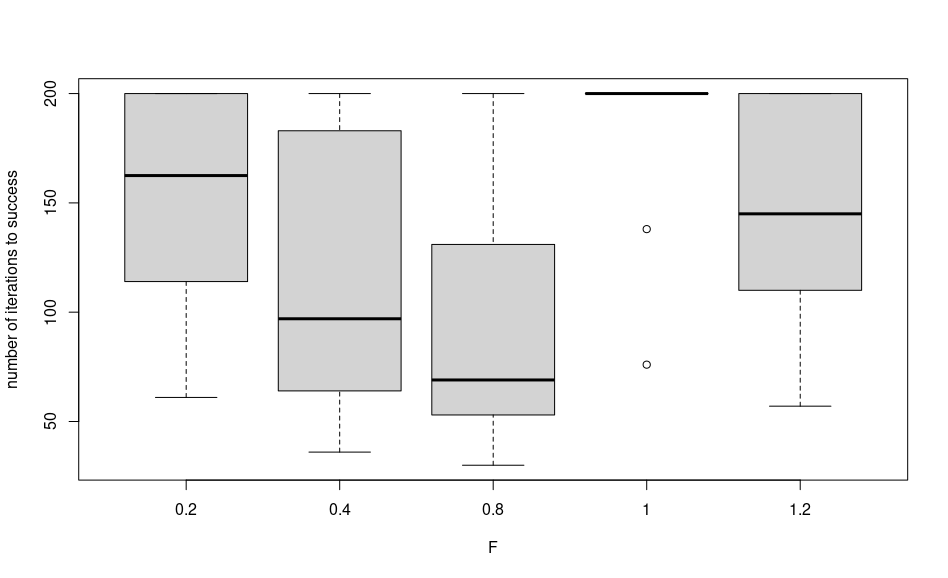
\includegraphics[width=\textwidth]{../img/DE_experiment_F_analysis.png}
  \end{columns}
\end{frame}

\begin{frame}[t,fragile]{Measuring Interaction Effect with a linear regression}{}

{\smaller
\begin{verbatim}
> DE.lm <- lm(formula = R ~ F + CR + F*CR,            <-- Linear Reg Formula
              data = tab.results)                         Includes F*CR, the
> summary(DE.lm)                                          iteraction factor.
(...)
Residuals:
    Min      1Q  Median      3Q     Max 
-90.107 -36.083   7.101  31.577 103.793               <-- Residuals don't look
(...)                                                     too skewed.
Coefficients:
            Estimate Std. Error t value Pr(>|t|)    
(Intercept)   212.31      12.94  16.409  < 2e-16 ***  
F             -13.15      15.97  -0.823  0.41124      <-- no "linear" effect!
CR           -177.01      22.52  -7.859 1.21e-13 ***
F:CR           74.56      27.81   2.681  0.00783 **   <-- Detects a significant
(...)                                                     effect from changing
                                                          both factors together
\end{verbatim}}                                                 
\end{frame}

\begin{frame}[t,fragile]{Interaction Graph -- CR by F}{}
  A visual investigation of interaction effects might be more informative.
\begin{verbatim}
interaction.plot(tab.results$CR, tab.results$F, tab.results$R)
\end{verbatim}

  \begin{columns}
    \column{0.6\textwidth}
    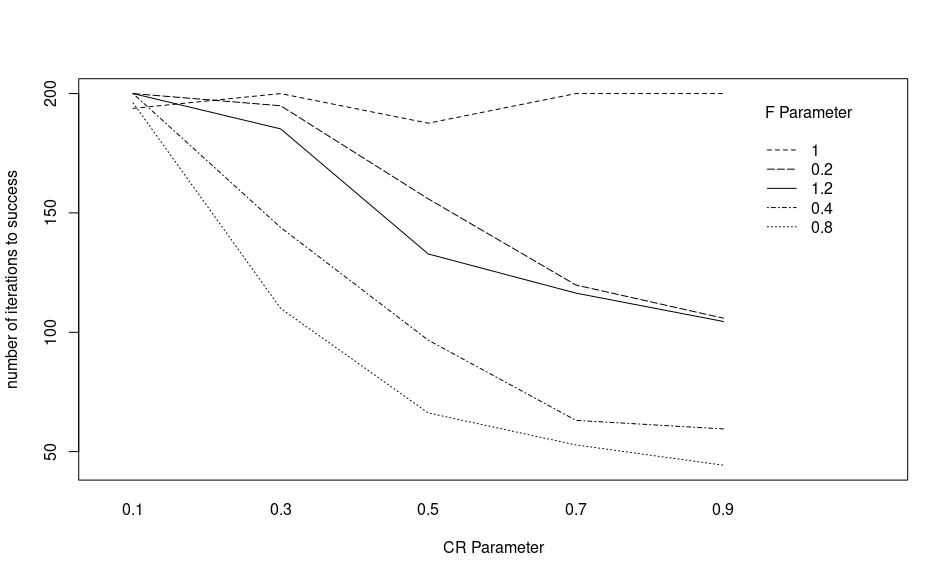
\includegraphics[width=\textwidth]{../img/interaction_DE_CRbyF.png}
    
    \column{0.4\textwidth}
    \begin{itemize}
    \item $F=0.2$ and $F=1.2$ show low convergence compared to $F=0.4$
      and $F=0.8$. But the shape of the curve seems roughly similar.
    \item Again we see the anomalous behavior of $F=1$
    \end{itemize}
  \end{columns}
\end{frame}

\begin{frame}[t,fragile]{Interaction Graph -- F by CR}{}
  A visual investigation of interaction effects might be more informative.
\begin{verbatim}
interaction.plot(tab.results$F, tab.results$CR, tab.results$R)
\end{verbatim}

  \begin{columns}
    \column{0.6\textwidth}
    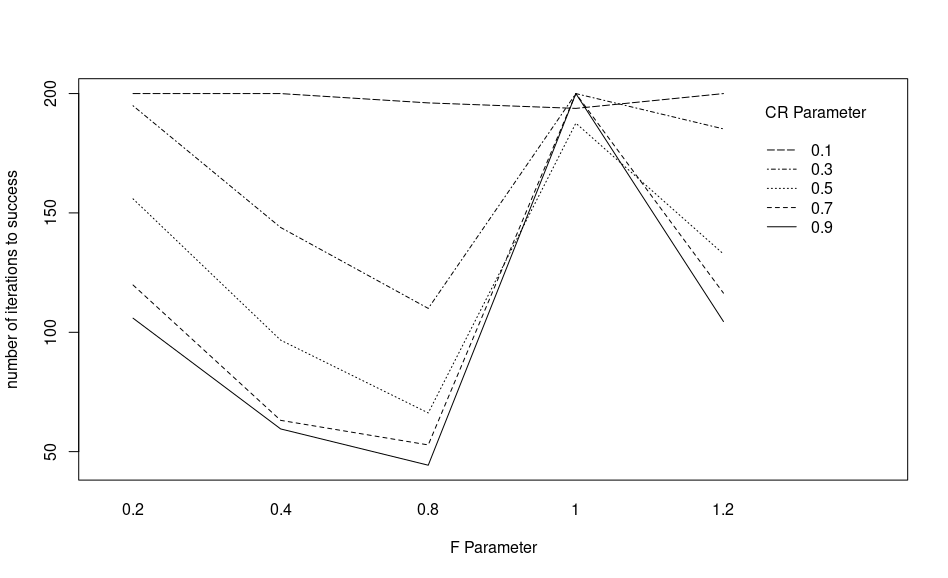
\includegraphics[width=\textwidth]{../img/interaction_DE_FbyCR.png}
    
    \column{0.4\textwidth}
    \begin{itemize}
    \item Here we see that the curves show roughly the same shape,
      and convergence speed increasing as CR increases;
    \item Here the anomalous behavior of $F=1$ is more pronounced.
    \end{itemize}
  \end{columns}
\end{frame}

\begin{frame}[t]{Early Conclusions}
  \begin{itemize}
  \item The linear regression model indicates a strong effect for a CR*F factor.\medskip
    
  \item However, this effect is not so clear in a visual inspection.
    \begin{itemize}
    \item This may be because the relationship between F and the
      output variable is not linear.
    \end{itemize}\medskip
    
  \item The recommendation {\bf from these results} would be to try
    $F=0.8$, and $CR$ as high as possible.
    \begin{itemize}
    \item Maybe worth investigation $CR > 0.9$;
    \end{itemize}\medskip
    
  \item Maybe worth it investigating $F = 1.0$ for bugs in the code,
    since a scaling factor should not have such an anomalous behavior.
    \bigskip
    
  \item \structure{A good experiment many times raises as many
      questions as it answers!}
    
  \end{itemize}
\end{frame}

\begin{frame}[t]{Caveats of this case study}{}
  \begin{itemize}
  \item {\bf Non-linear effects}: $F$ shows a clear non-linear
    relationship with the output variable.
    \begin{itemize}
    \item Note how the difference cause the linear model to return
      non-reliable information!
    \item Good opportunity to investigate non-linear models.
    \end{itemize}\bigskip

  \item Second order interaction is already though. Third order
    interaction and above become exponentialy harder to analyze;
    \bigskip

  \item Eventually, it becomes more practical to use sequential models
    like IRACE and SMAC;
  \end{itemize}
\end{frame}


\begin{frame}{Suggested Extra Reading}{}
  \begin{itemize}
  \item Bartz-Bielstein: ``Experimental Methods for the Analysis of
    Optimization Algorithms'', In depth discussion about
    parametrization and analysis of algorithms like DE;\bigskip

  \item Paul Teetor: ``R Cookbook'', Quick recipes for a variety of
    data visualizations in R;\bigskip
    
  \item Statistics by Jim: ``Interaction Effects''.\\
    A short, intuitive description of interaction
    effects. \url{https://statisticsbyjim.com/regression/interaction-effects/}
    \bigskip
    
  \item T.J. VanderWeele, M. J. Know: ``A Tutorial on Interaction.\\
    A more in-depth discussion of interaction in several models, but focused on medicine use cases.
    \url{https://www.hsph.harvard.edu/wp-content/uploads/sites/603/2018/04/InteractionTutorial_EM.pdf}
  \end{itemize}
\end{frame}

%%% Notes
% Interaction effects are common in regression models,
% Anova, and designed experiments
% Interaction plot -- (of two variables)



% Categorical Variables
% Continuous independent variables




%%% Local Variables:
%%% mode: latex
%%% TeX-master: "topic08"
%%% End:

\section{Equality Testing}

\begin{frame}

  \begin{center}
    {\bf Part I -- Equality Testing}
  \end{center}

\end{frame}

\begin{frame}{Testing equivalence}{Introduction}

In the previous lectures, we introduced tests that focus on detecting {\bf differences} between a population parameter $\theta$ and its nominal value $\theta_0$ under a null hypothesis.\bigskip

In engineering and science, we are sometimes interested in investigating the {\bf equivalence}, within a given margin of error. Some example cases:\bigskip

\begin{itemize}
  \item Conformity/compliance testing (industrial certification);
  \item Equivalence of effects (pharmaceutical industry);
\end{itemize}
\end{frame}

\begin{frame}{Testing equivalence}{Question of interest in usual studies}
In principle, one could express this as a shift in focus from trying to establish whether a population parameter is different from a given reference to trying to determine whether it is equal to that reference.
\vfill

In usual (two-sided) comparative studies, the {\bf alternative hypothesis} (i.e., the one that presents novelty in relation to the current state of knowledge) is the one of difference between the parameters of interest - that is, unless there is strong evidence of differences, one cannot rule out the null hypothesis of equality;
\end{frame}

\begin{frame}{Testing equivalence}{Question of interest in equivalence studies}
In equivalence testing, the situation is reversed: the (approximate) equality of two parameters is the novelty one hopes to establish. Consequently, the burden of proof shifts to providing evidence that there is no difference.
\bigskip

The term \textit{equivalent} is not used strictly, but to mean the absence of practical differences - that is, any differences that might exist fall within an \textit{equivalence margin} or \textit{limit of practical significance} $\delta^*$.
\bigskip

Using this approach, the equivalence of two parameters can be established if a sample provides enough evidence that the true difference is smaller than $\delta^*$ units.
\end{frame}

\begin{frame}{Testing Non-inferiority}{Equivalence and non-inferiority}
A similar concept to equivalence testing is the definition of non-inferiority of a given treatment/ process/ method in relation to another (e.g., a standard solution).
\bigskip

In non-inferiority tests, one can declare that a given process is not worse than a standard one only if enough evidence is provided to conclude that the performance of the proposed process is no more than $\delta^*$ units worse than that of the standard.
\bigskip

In the case of non-inferiority tests, one can in principle use a regular test of differences with a one-sided alternative (which would be equivalent to setting $\delta^* = 0$), or define the null hypothesis in a way that includes $\delta^*$ in its formulation.
\end{frame}


\begin{frame}{Comparison of studies}
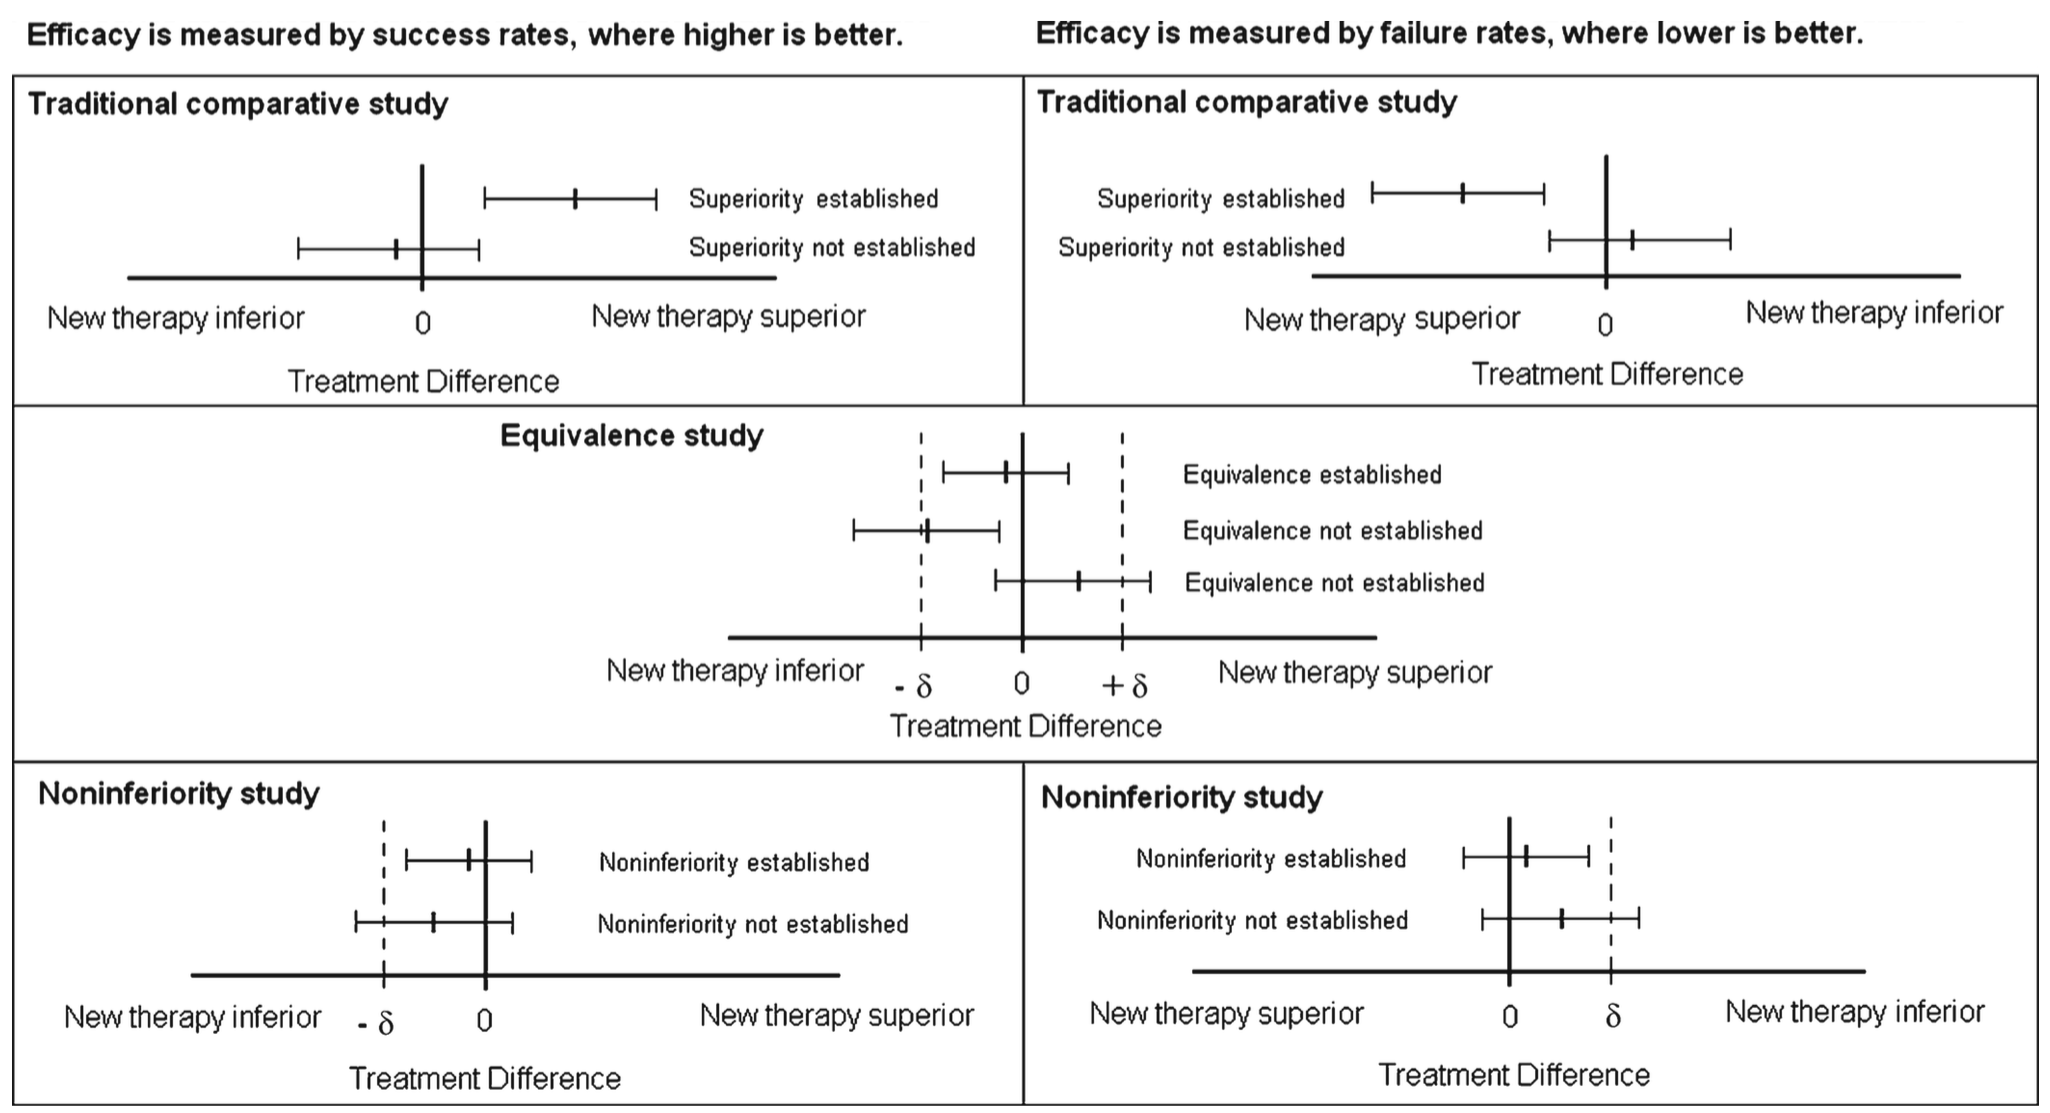
\includegraphics[width=\textwidth]{../img/TOST.png}
\ppagenote{Summary of Equivalence Testing: Walker and Nowacki (2011), J. General Internal Medicine 26(2):192-196.}
\end{frame}


\begin{frame}{Testing Equivalence}{Quick-and-dirty approach}
A simple way of thinking about testing equivalence of two means is to observe confidence intervals instead of p-values:

\begin{exampleblock}{}
\centering ``\textit{Equivalence can be established at the $\alpha$ significance level if a $(1-2\alpha)$-confidence interval for the difference between the two means is contained within a interval $\pm\delta^*$.}''
\end{exampleblock}

The difference between testing for differences and for equivalence can be easily illustrated using this approach:

\centering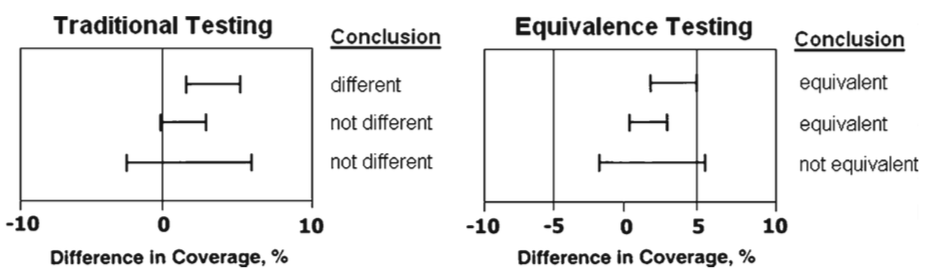
\includegraphics[width=.8\textwidth]{../img/DiffVxEquiv.png}
\ppagenote{Difference vs Equivalence Image: Walker and Nowacki (2011), J. General Internal Medicine 26(2):192-196.}
\end{frame}

\begin{frame}{Equivalence test for a single mean}{Hypotheses}
An equivalence test for a single population mean can be expressed by the hypotheses:
\begin{equation*}
  \begin{cases}
  H_0: \left|\mu-\mu_0\right| = &\Delta\mu \geq\delta^*\\
  H_1: &\Delta\mu <\delta^*
  \end{cases}
\end{equation*}
\medskip

The most usual way of testing these hypotheses is the TOST (\textit{two one-sided tests}) method. As the name suggests, two one-sided significance tests are constructed so that the desired statistical properties can be achieved. Using our standard notation:
\begin{columns}[T]
\column{0.5\textwidth}
\begin{equation*}
\begin{cases}
H_0^1: &\Delta\mu = -\delta^*\\
H_1^1: &\Delta\mu > -\delta^*
\end{cases}
\end{equation*}
\column{0.5\textwidth}
\begin{equation*}
\begin{cases}
H_0^2: &\Delta\mu = \delta^*\\
H_1^2: &\Delta\mu < \delta^*
\end{cases}
\end{equation*}
\end{columns}
\bigskip
If both tests reject their respective $H_0$, then equivalence (within the equivalence margin $\delta^*$) can be declared with significance level $\alpha$.
\end{frame}

\begin{frame}{Interpretation of the Two One Sided Hypothesis}
\centering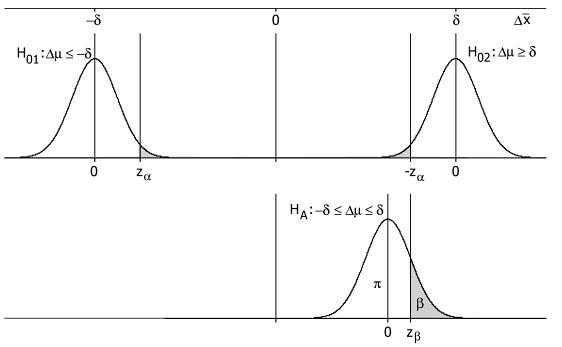
\includegraphics[width=.9\textwidth]{../img/TOST-errors.png}
\ppagenote{TOST errors image: Matthews (2010), Sample Size Calculations, MMB. pg. 46}
\end{frame}


%% Sample sizes
% \begin{frame}{Equivalence of a single mean}{Sample size}
% Sample sizes for testing equivalence of a single mean can be derived using essentially the same considerations used for the usual tests. In the case of a single sample:
% \begin{equation*}
% n\geq\left(\frac{\left(t_{\alpha}+t_{\beta}\right)\hat{\sigma}}{\delta^* - \Delta\mu}\right)^2
% \end{equation*}
% \bigskip
%
% As in the previous cases, iteration is needed to solve for $n$ (since the quantiles of the t distribution depend on $n$). Use $t_x$ = $z_x$ for the first iteration.
% \end{frame}


\begin{frame}{Equivalence Testing by TOST}{Hypotheses for two samples}
Analogously to the single sample test of equivalence, the hypotheses for testing the equivalence of two population means can be described as:
\begin{equation*}
\begin{cases}
H_0: &\mu_1-\mu_2 \geq\delta^*\\
H_1: &\mu_1-\mu_2 <\delta^*
\end{cases}
\end{equation*}
\hrulefill

\begin{columns}[T]
\column{0.5\textwidth}
\begin{equation*}
\begin{cases}
H_0^1: &\mu_1-\mu_2 = -\delta^*\\
H_1^1: &\mu_1-\mu_2 > -\delta^*
\end{cases}
\end{equation*}
\column{0.5\textwidth}
\begin{equation*}
\begin{cases}
H_0^2: &\mu_1-\mu_2 = \delta^*\\
H_1^2: &\mu_1-\mu_2 < \delta^*
\end{cases}
\end{equation*}
\end{columns}
\bigskip

Just as in the previous case, both hypotheses are tested at the desired $\alpha$ value, and the rejection of both $H_0$ indicates evidence of equivalence.
\end{frame}



% \begin{ftst}
% {Equivalence of two means}
% {Sample size}
% Sample size for the $n_1 = n_2 = n$ case can be approximated based on the Zhang formula\footnote[1]{\tiny Zhang (2003), J. Biopharm. Stat. 13(3):529-538.}:
% $$n \geq \left(t_{\alpha;\nu}+t_{(1-c)\beta;\nu}\right)^2\left(\frac{\hat{\sigma}_1^2+\hat{\sigma}_2^2}{\delta^*-\Delta\mu^*}\right)^2$$
%
% \noindent with $\Delta\mu^*<\delta^*$ as the maximum real difference between the two means for which a power of $(1-\beta)$ is desired, and:
% $$c = \frac{1}{2}\exp\left(-7.06\frac{\Delta\mu^*}{\delta^*}\right)$$
%
% The degrees of freedom $\nu$ of the t-quantiles are given by the Welch t-test formula (see Chapter 6).
% \end{ftst}
%
% %=====
%

\subsection{Example}

\begin{frame}{Example -- Laboratory certification}

\begin{columns}[T]
  \column{0.7\textwidth}
  A ballistics laboratory is in the process of being certified for the evaluation of shielding technology, and needs to provide evidence of equivalence of a given callibration procedure with the reference equipment;
  \column{0.3\textwidth}
  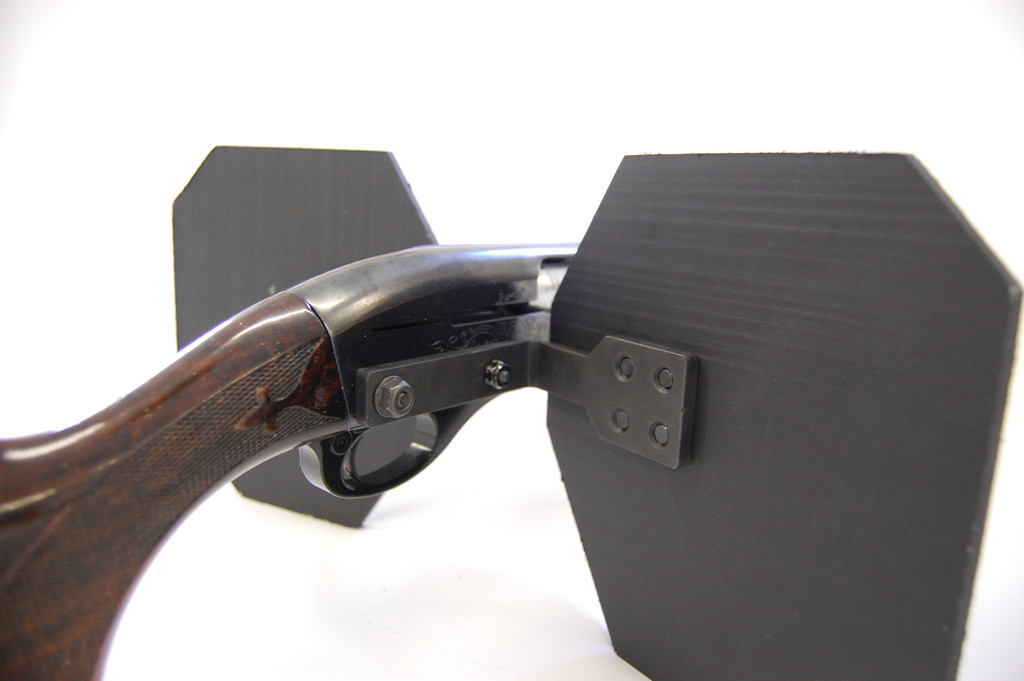
\includegraphics[width=\textwidth]{../img/Shotgun-Ballistic-Shield.png}
  \ppagenote{Gun Shield Image from: \url{http://www.everydaynodaysoff.com/2013/08/05/ballistic-shield-for-operators-only/}}
\end{columns}
\bigskip

The certification authority demands that the mean hole area generated by this procedure in the lab be the same as the one from the reference equipment, and tolerates deviations no greater than $4 mm^2$;
\bigskip

From previous measurements, the standard deviations can be roughly estimated as $\hat{\sigma}_{Lab} = 5 mm^2$ and $\hat{\sigma}_{ref} = 10 mm^2$.
\bigskip

The desired error levels for the comparison are $\alpha=0.01$ and $\beta = 0.1$.
\end{frame}

\begin{frame}[fragile]{Example -- Laboratory certification}
To calculate the required sample size, assume that $\Delta\mu^* = 0.5$. Then:
\begin{verbatim}
> # load functions to calculate sample size for TOST
> source("calcN_tost.R")
>
> # Calculate sample size
> calcN_tost2(alpha = 0.01,
+             beta = 0.1,
+             diff_mu = 0.5,
+             tolmargin = 4,
+             s1 = 5,
+             s2 = 10)
[1] 144.1999
\end{verbatim}
\medskip
We'll need 145 observations from each group to test for equivalence with the desired experimental properties.
\end{frame}

\begin{frame}[fragile]{Certification -- Data Analysis}
After collecting the observations, we proceed to the analysis:
{\tiny
\begin{verbatim}
> data<-read.table("../data files/labdata-example.csv",
+                  header = T, sep = ",")

> # Two one-sided t-tests
> t.test(HoleArea~Place,  data = data,  alternative = "less", mu = 4,
+        conf.level = 0.99)$p.value
[1] 0.00304124
> t.test(HoleArea~Place, data = data, alternative = "greater", mu = -4,
+        conf.level = 0.99)$p.value
[1] 6.586193e-10

> # Get (1-2*alpha) CI
> t.test(HoleArea~Place, data = data,  conf.level = 0.98)$conf.int
[1] -0.5117627  3.6244386
\end{verbatim}}

\hfill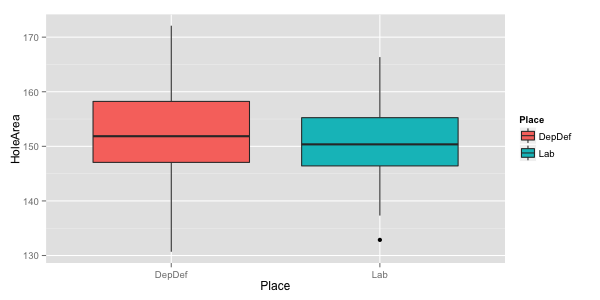
\includegraphics[width=.45\textwidth]{../img/labdata.png}
\end{frame}


\begin{frame}[fragile]{Verification of test assumptions -- Normalty}
\hfill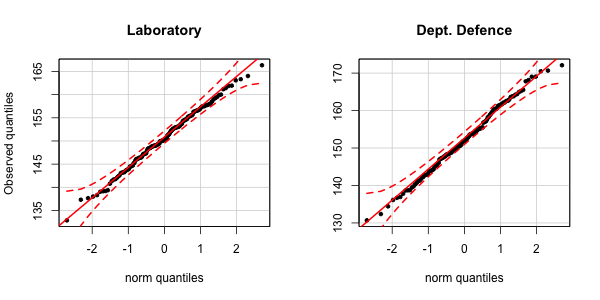
\includegraphics[width=.6\textwidth]{../img/labdata-qqplots.png}
{\smaller
\begin{verbatim}
> par(mfrow=c(1,2))
> qqPlot(subset(data, Place=="Lab")[,2],
+        pch=20,
+        main = "Laboratory",
+        ylab = "Observed quantiles")
> qqPlot(subset(data, Place=="DepDef")[,2],
+        pch=20,
+        main = "Dept. Defence",
+        ylab = " ")
\end{verbatim}}
\end{frame}

\begin{frame}[fragile]{Verification of test assumptions -- Independence}

{\smaller
\begin{verbatim}
> dwtest(HoleArea~Place, data=data)
DW = 1.8116, p-value = 0.04757

> par(mfrow=c(1,2))
> plot(seq_along(subset(data, Place=="Lab")[,2]),
+      subset(data, Place=="Lab")[,2], ...)
> plot(seq_along(subset(data, Place=="DepDef")[,2]),
+      subset(data, Place=="DepDef")[,2], ...)
\end{verbatim}}

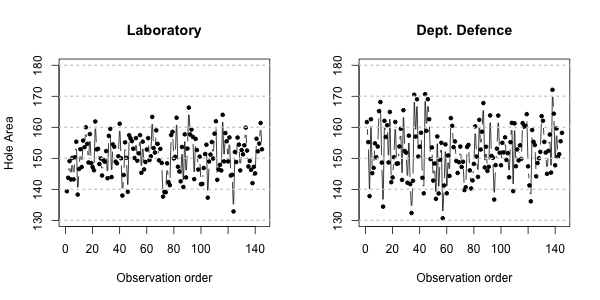
\includegraphics[width=.7\textwidth]{../img/labdata-resplot.png}
\end{frame}

%\section{Correlation Testing}

\begin{frame}{}

  \begin{center}
    {\large {\bf
        Testing for correlation
    }}
  \end{center}
  
\end{frame}

\begin{frame}{General Idea}
\end{frame}



%%% Local Variables:
%%% mode: latex
%%% TeX-master: "topic08"
%%% End:

%\section{Variance Comparison}

\begin{frame}{}

  \begin{center}
    {\large {\bf
        Comparing the Variance of two Samples
    }}
  \end{center}
  
\end{frame}

\begin{frame}{General Idea}
\end{frame}

%\section{Recommended Reading}
%\begin{frame}{Recommended Reading}
  
%\end{frame}

%%%%%%%%%%%%%%%%%%%%%%%%%%%%%%%%%%%%%%%%%%%%%%%%%%%%
\section{Backmatter}
\begin{frame}{About these Slides}
  These slides were made by Claus Aranha, 2022. You are welcome to copy, re-use and modify this material.
  \bigskip

  These slides are a modification of "Design and Analysis of Experiments (2018)" by Felipe Campelo, used with permission.
  \bigskip

  Individual images in some slides might have been made by other
  authors. Please see the following references for those cases.
\end{frame}

\begin{frame}[allowframebreaks]{Image Credits}
  \printnotes
\end{frame}

\end{document}

%%% Local Variables:
%%% mode: latex
%%% TeX-master: t
%%% End:
